\documentclass[9pt,xcolor=dvipsnames]{beamer}
\usepackage[latin1]{inputenc}
\usepackage[spanish]{babel}
\usepackage{verbatim}
\usepackage{natbib}
\usepackage{mathptmx}
%\usepackage{beamerthemesplit}
\usepackage{multirow}
\usepackage{amsmath,amsfonts,amssymb,amsthm}
\usepackage{graphicx}
\usepackage{bbold}
\setbeamertemplate{caption}[numbered]
\usepackage{listings}  % para incluir c�digo en las diapositivas, ojo, hay que incluir [fragile] en esas diapositivas

\lstset{ 
  language=R,                     % the language of the code
  basicstyle=\small\ttfamily,     % the size of the fonts that are used for the code
  numbers=left,                   % where to put the line-numbers
  numberstyle=\small\color{Blue}, % the style that is used for the line-numbers
  stepnumber=1,                   % the step between two line-numbers. If it is 1, each line
                                  % will be numbered
  numbersep=5pt,                  % how far the line-numbers are from the code
  backgroundcolor=\color{white},  % choose the background color. You must add \usepackage{color}
  showspaces=false,               % show spaces adding particular underscores
  showstringspaces=false,         % underline spaces within strings
  showtabs=false,                 % show tabs within strings adding particular underscores
  rulecolor=\color{black},        % if not set, the frame-color may be changed on line-breaks within not-black text
  tabsize=3,                      % sets default tabsize to 2 spaces
  captionpos=b,                   % sets the caption-position to bottom
  breaklines=true,                % sets automatic line breaking
  breakatwhitespace=false,        % sets if automatic breaks should only happen at whitespace
	xleftmargin=1cm,
  keywordstyle=\color{RoyalBlue},      % keyword style
  commentstyle=\color{YellowGreen},    % comment style
  stringstyle=\color{ForestGreen}      % string literal style
} 


\usetheme{Madrid}



\parskip 3mm
\usefonttheme[onlylarge]{structuresmallcapsserif}
\usefonttheme[onlysmall]{structurebold}



\title[Introducci\'on a la Estad\'istica Computacional]{Introducci\'on a la Estad\'istica Computacional}
%\subtitle{Taller de Simulaci\'on}
\author[R. \'Alvarez-Vaz- G. Berm\'udez]{Ram\'on \'Alvarez-Vaz;Gabriel Berm\'udez}
%\institute[IESTA]{Instituto de Estad\'istica}
\titlegraphic{
\includegraphics[width=10cm]{grafi/LOGO_DMC}}
\date{Mi�rcoles 19 de agosto 2026}


\begin{document}
% para poner p-valor menor a 0.001
\newcommand{\pvu}{$\textless0.001$}
% color amber
\definecolor{amb}{rgb}{1,0.49,0}
% para modificar el espacio sobre y debajo de las ecuaciones
\abovedisplayskip=2mm
\belowdisplayskip=-2mm
% para modificar el espacio sobre y debajo de las figuras
\abovecaptionskip=2mm
\belowcaptionskip=-2mm

\begin{frame}[plain]
	\titlepage
\end{frame}


\begin{frame}
\frametitle{Aspectos Reglamentarios}

\begin{block}{Clases}
	Mi\'ercoles y Viernes  de 10:00 a 12:00.\\
	Exposiciones te\'orico-pr\'acticas y algunos d\'ias exclusivamente dedicados a la realizaci\'on de ejemplos, problemas y ejercicios en R.
\end{block}

\pause

\begin{block}{Docentes}
		Ram\'on \'Alvarez-Vaz\\
		Gabriel Berm\'udez.

\end{block}

\pause

\begin{block}{Bibliograf\'ia}
	Adem\'as de las transparencias de cada clase:\\
	\begin{itemize}
		\item \emph{Introduction to scientific programming and simulation using R}. - Jones, Maillardet y Robinson.\cite{jones2014}\\
	\end{itemize}
	
	\pause
	
	Y para algunos temas pueden consultar:\\
	\begin{itemize}
		\item \emph{Introducing Monte Carlo methods with R}. - Robert y Casella,\cite{robert2010}\\
		\item \emph{Using R for numerical analysis in science and engineering}. - Bloomfield\cite{Bloomfield2014}\\
		\item \emph{Numerical Optimization}. - Nocedal y wright, \cite{nocedal2006}\\
	\end{itemize}
\end{block}
\end{frame}


\begin{frame}
\frametitle{Ganancia del Curso}

Las evaluaciones ser\'an las siguientes:

\pause

\begin{itemize}
	\item Una revisi\'on (30pts).
	\item Una carpeta de ejercicios (20pts).
	\item Una Entrega final (40pts).
	\item Evaluaci\'on individual de la	exposici\'on del trabajo grupal (10pts).
\end{itemize}

\pause

�C\'omo exonero la parte escrita del examen?

\pause

\begin{itemize}
	\item Obteniendo al menos 15 de los 30 puntos de la revisi�n.
	\item Obteniendo al menos 10 de los 20 puntos de la carpeta.
	\item Obteniendo al menos 20 de los 40 pts del Trabajo final.
	\item Obteniendo al menos 5 de los 10 pts de la exposici�n del trabajo en grupo.
	\item \textcolor[rgb]{1,0,0}{Obteniendo al menos 50 pts entre los tres anteriores.}
\end{itemize}

\end{frame}



\begin{frame}
\frametitle{Temas}

El curso se dividir\'a en dos grandes partes:
\pause

\begin{block}{M\'etodos Computacionales}
	\begin{itemize}
		\item Errores.
		\item Estructuras de Control.
		\item Ceros de funciones.
		\item Optimizaci�n num\'erica.
		\item Integraci�n num\'erica.
	\end{itemize}
\end{block}

\pause

\begin{block}{Simulaci\'on}
	\begin{itemize}
		\item Generaci\'on de variables aleatorias.
		\item Reducci\'on de varianza.
		\item Integraci\'on de Monte-Carlo.
		\item Bootstrap (si nos alcanza el tiempo).
	\end{itemize}
\end{block}
\end{frame}


\begin{frame}
\frametitle{Requerimientos}

\begin{block}{Previaturas}
Si bien se requiere contar con Probabilidad I, se valorar\'a contar con conocimientos de Inferencia I. Sobre todo cuando se llegue al cap\'itulo de optimizaci\'on.
\end{block}

\pause

Adicionalmente, se valorar\'a conocimiento del software R. Sin embargo, se espera que con este curso el estudiante ahonde en su manejo del programa orientado a la programaci\'on cient\'ifica.

\pause
Aquellos que hayan cursado \emph{M\'etodos Num\'ericos} en Fing notar\'an algunas similitudes en los contenidos. Sin embargo, este curso est\'a orientado a la aplicaci\'on de t\'ecnicas computacionales en el \'ambito de la estad\'istica.

\end{frame}

\begin{frame}
\frametitle{Porqu\'e Introducci\'on a la Estad\'istica Computacional?}  
\begin{block}{complementos de los temas}
	\begin{itemize}
		\item Cursos de c\'alculo o an\'{a}lisis num\'{e}rico  de otras carreras de grado de la Udelar.
		\item Presentaci\'{o}n de algunos problemas de la vida real que a poco de razonar nos llevan a tener que usar para su resoluci\'{o}n una serie de t\'{e}cnicas de aproximaci\'{o}n, de
		simulaci\'{o}n en el sentido m\'as amplio y obviamente el uso de alguna
		herramienta inform\'{a}tica.
		\item Actualmente es impensable tratar de hacer c\'{a}lculos estad\'{i}sticos
		medianamente complejos sin usar una herramienta inform\'{a}tica como puede
		ser un lenguaje de programaci\'{o}n de alto nivel paquete estad\'{i}stico (R, Matlab, Octave, C, Fortran, Python, Julia).
		\item Por ese motivo deberemos tratar de resolver
		nuestros problemas en cuesti\'{o}n con la ayuda de la computadora y teniendo
		por lo tanto que aprender a entender cual es la \emph{''matem\'{a}tica''}
		que esta usa y que veremos se diferencia bastante de los que podemos haber
		aprendido en nuestros cursos de c\'{a}lculo diferencial e integral, de \'{a}lgebra lineal, etc.
	\end{itemize}
\end{block}
\end{frame}

\begin{frame}
\frametitle{Ejemplo 1 (1)}  
\begin{block}{Tratamos de Sumar y.....}
	Supongamos que deseamos obtener la suma
	
	\begin{equation}
	\sum_{k=1}^{k=300000} \frac{1}{30}
	\end{equation}
	
	A priori sabemos cuanto debe dar esa suma, que consiste en sumar 300000
	veces 1/30, cuya respuesta es 10000. Sin embargo cuando deseemos evaluar la
	suma con el uso de una computadora veremos que las cosas no son tan
	f\'{a}ciles ya que podemos tener como resultado
	
	\begin{equation}
	\sum_{k=1}^{k=300000}  \frac{1}{30}=10000.0000000228\text{ \ \ \ \ \ \ \ \ \ \ \
		!!!!!!!!!!!!!!!!!!!!}
	\end{equation}
	\pause
Como puede darse esta situaci\'{o}n? Muy sencillo ya que nuestra respuesta
de 10000 es v\'{a}lida en la medida en que nosotros estamos acostumbrados a
manejarnos usando el sistema decimal mientras que las computadoras hacen sus c\'{a}lculos en el sistema binario (en base 2)	
\end{block}
\end{frame}

\begin{frame}[fragile]
\frametitle{Ejemplo 1 (2)}  
\begin{block}{Veamos porqu\'e}
	{\footnotesize 
		\begin{verbatim}
		k<-300000
		sumando<-1/30
		str(sumando)
		suma<-0
		for (i in 1:k)
			{
			suma<-suma+sumando
			}
		compara=sumando*k
		compara==suma
		[1] FALSE
		all.equal(compara,suma,tolerance = 1.5e-12)
		[1] "Mean relative difference: 2.277557e-12"
		all.equal(compara,suma)
		[1] TRUE
		signif(suma,10)
		round(suma,10)
		suma-compara
		\end{verbatim}
	}

\pause
Vemos entonces que algo tan sencillo como una suma de t\'{e}rminos constantes se calcula en forma diferente a como lo har\'{i}amos en forma manual, por lo que podemos hacernos una idea de c\'{o}mo ser\'{a} la situaci\'{o}n cuando debamos evaluar integrales, derivadas, determinantes.

\end{block}

\end{frame}

\begin{frame}
\frametitle{ Ejemplo 2}  
\begin{block}{Evaluaci\'on de Polinomios}
Algo tan sencillo como evaluar un \emph{polinomio de grado n} \citep{Mathews2004}
que se presenta como una \emph{Combinaci\'on  Lineal de n+1} t\'{e}rminos, se puede resolver de forma m\'{a}s sencilla usando un poco el ingenio 

\begin{equation}
P(x)=a_{n}x^{n}+a_{n-1}x^{n-1}+a_{n-2}x^{n-2}........+a_{2}x^{2}+a_{1}x^{1}+a_{0}
\end{equation}

\begin{itemize}
	\item Evaluar $P(c)$ implica hacer una cuantas operaciones (calcular las diferentes potencias de x, multiplicarlas por sus respectivas coeficientes y luego evaluar la suma. Sin embargo podemos hacer casi la mitad de las operaciones con solo factorizar mediante multiplicaciones encajadas
	\pause
	\item Para un polinomio de grado 5 tenemos $%
	P(x)=a_{5}x^{5}+a_{4}x^{4}+a_{3}x^{3}+a_{2}x^{2}+a_{1}x^{1}+a_{0 }$
	
	\pause
	\item Si factorizamos tenemos $	P(x)=((((a_{5}x + a_{4})x+a_{3})x+a_{2})x+a_{1})x+a_{0}$ vemos que es mucho m\'{a}s sencillo de calcular .
	
	\item Vamos viendo entonces que no solo se trata de ver que calcular a veces es
	una cuesti\'{o}n de estrategia!!!!! 
	
\end{itemize}
\end{block}
\end{frame}

\begin{frame}
\frametitle{Ejemplo 3 (1)}  
\begin{block}{Ceros de funciones o Ra\'ices de Ecuaciones No lineales}
Supongamos que tenemos una Variable Aleatoria con funci\'on de distribuci\'on conocida
$F_X (x)$. 
\begin{itemize}
	\item Si tuvi\'esemos necesidad de encontrar el percentil alfa-\'esimo, lo que tendremos que calcular es 
	\[F_X (x) = \alpha \]
	o lo que es lo mismo 
	\[F_X (x) - \alpha=0 \]
	\item 	Muchas veces  $F_X (x)$ puede tener una expresi\'on complicada para evaluar, por lo tanto resolver la integral no se puede hacer anal\'iticamente. 
	\item Una posibilidad es resolver la ecuaci\'on antes planteada.
\end{itemize}
\end{block}
\end{frame}


\begin{frame}
\frametitle{Ejemplo 3 (2)}  
\begin{block}{Proyecto de Inversiones}
Supongamos que tenemos un   proyecto de inversi\'{o}n tal cual aparece en la figura que sigue.

En ese caso el  Valor Presente Neto (VPN) es

\begin{equation}
VPN =  - I_0  + \sum\limits_{k = 1}^{k = n} {\frac{{I_k }}{{(1 + i)^k }}} 
\end{equation}
\pause
A partir del VPN , nosotros podemos estar interesados en calcular la tasa de inter\'es a la que se reproducen los fondos.\\

Es decir que esa tasa, que es la Tasa Interna de Retorno (TIR)  es la que verifica

\begin{equation}
VPN =  - I_0  + \sum\limits_{k = 1}^{k = t} {\frac{{I_k }}{{(1 + i)^k }}}=0 
\end{equation}

Entonces estamos nuevamente enfrentados a tener que resolver , en este caso la ecuaci\'on $f(x)=0$, con $f(x)$ un funci\'on polin\'omica de grado $t$ en \textbf{$(1+i)$}

\end{block}
\end{frame}


\begin{frame}
\frametitle{Ejemplo 3 (3)}  

\begin{figure}[htbp]
	\centering
	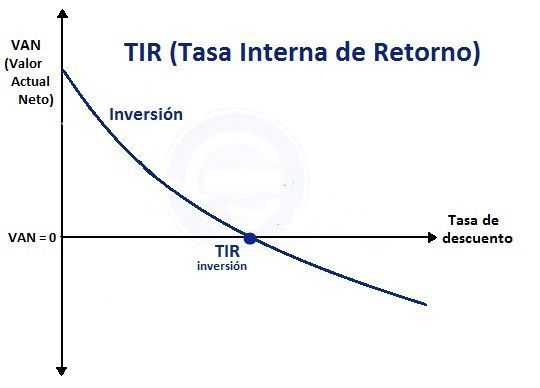
\includegraphics[width=0.60\textwidth]{grafi/TIR.jpg}
	\label{fig:TIR}
	\caption{Tasa Interna de Retorno. fuente: https://economipedia.com/definiciones/tasa-interna-de-retorno-tir.html
}
\end{figure}

\end{frame}
\begin{frame}
\frametitle{Ejemplo 3 (4)}  

\begin{figure}[htbp]
	\centering
	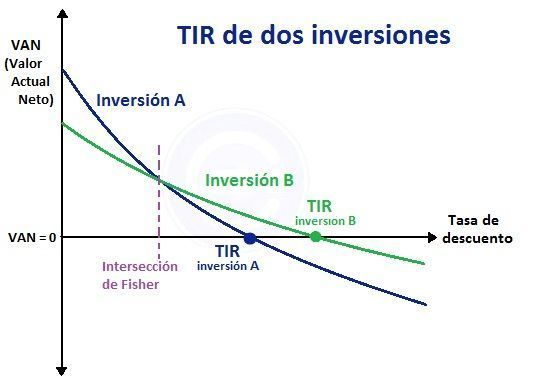
\includegraphics[width=0.60\textwidth]{grafi/TIR_2.jpg}
	\label{fig:TIR_2}
	\caption{Tasa Interna de Retorno para 2 proyectos. fuente: https://economipedia.com/definiciones/tasa-interna-de-retorno-tir.html
	}
\end{figure}

\end{frame}

\begin{frame}
\frametitle{Ejemplo 3 (5)}  
\begin{block}{Modelos de crecimiento}
	Hay problemas vinculados al crecimiento de poblaciones, en el campo de la \textbf{Biolog\'ia} y de la \textbf{Demograf\'ia} cuya soluci\'on se basa en la resoluci\'on de ecuaciones diferenciales o de ecuaciones no lineales.\\
	
	Supongamos que tenemos una poblaci\'on que var\'ia en el tiempo, es decir que tenemos $N(t)$ cantidad de individuos en $t$ y si suponemos que la velocidad de cambio de la poblaci\'on es proporcional a una constante y a la poblaci\'on en un momento dado nos queda una ecuaci\'on diferencial como sigue:
	
	\begin{equation}
	\label{eq:modelo}
	\frac{{dN(t)}}{{dt}} = N(t)\lambda 
	\end{equation}
	La ecuaci\'on \eqref{eq:modelo} se puede resolver y nos queda el siguiente planteo:
	
	\begin{eqnarray}
	\begin{array}{l}
	\int\limits_o^t {\frac{{dN(t)}}{{dt}}}  = \int\limits_0^t {N(t)\lambda }  \\ 
	\Rightarrow Ln(N(t)) - Ln(N(0)) = \lambda t - \lambda 0 \\ 
	\Rightarrow Ln\left[ {\frac{{N(t)}}{{N(0)}}} \right] = \lambda t \\ 
	\end{array}
	\end{eqnarray}
	
\end{block}
\end{frame}

\begin{frame}
\frametitle{ Ejemplo 3 (6)}  
\begin{block}{Soluci\'on}

\begin{equation}
\frac{{N(t)}}{{N(0)}} = e^{\lambda t}  \Rightarrow N(t) = N(0)e^{\lambda t} \Rightarrow N(t)- N(0)e^{\lambda t}=0
\end{equation}

Una variante de este modelo de crecimiento es si suponemos que existen adem\'as par\'ametros que regulan la entrada o salida (inmigraci\'on o emigraci\'on). En ese caso lo que tenemos es de la forma:

\begin{eqnarray}
\begin{array}{l}
\frac{{dN(t)}}{{dt}} = N(t)\lambda  +  \nu  \\ 
\Rightarrow N(t) = N(0)e^{\lambda t}  + \frac{\nu }{\lambda }(e^{\lambda t}  - 1) \\ 
\end{array}
\end{eqnarray}
\\
En ese caso suponiendo que conocemos $N(0),\lambda,\nu$ y $N(1)$ otra forma de plantear es: 

\begin{eqnarray}
\begin{array}{l}
N(1) + \frac{\nu }{\lambda } = \left( {N(o) + \frac{\nu }{\lambda }} \right)e^\lambda   \\ 
\Rightarrow N(1) - N(0)e^\lambda   - \frac{\nu }{\lambda }(e^\lambda   - 1) = 0 \\ 
\end{array}
\end{eqnarray}
\end{block}
\end{frame}

\begin{frame}
\frametitle{Ejemplo 4}  
\begin{block}{Resolviendo Integrales Funciones de Distribuci\'on}
\begin{itemize}
	\item Tenemos la siguiente funci\'{o}n de densidad ,$f(x)=\frac{e^{-\lambda
		x}\lambda ^{n}x^{n-1}}{\Gamma (n)}$ para $0\leq x\leq \infty $ \ donde $\Gamma (n)$ es la funci\'{o}n \ gamma $\Gamma (n)=\int_{0}^{\infty
}e^{-x}x^{n-1}dx\quad $ Como vemos tenemos que evaluar 2 integrales.


\item 
Mas frecuente a\'un el caso de que $f(x)=\frac{1}{\sigma \sqrt{2\pi }}\exp %
\left[ \frac{-1}{2}\left( \frac{x-\mu }{\sigma }\right) ^{2}\right] $ que no
es m\'as que la ya conocida Variable Aleatoria Normal o lo que es lo mismo $x\sim N(\mu
,\sigma ^{2}).$

\item En este caso tenemos una integral que no se puede resolver mediante los m\'{e}todos convencionales vistos en nuestros cursos de c\'{a}lculo, con lo que deberemos lidiar con nuestra computadora que calcula en base 2 una soluci\'{o}n aproximada a la integral que queremos evaluar.
\end{itemize}
\end{block}
\end{frame}

\begin{frame}
\frametitle{Ejemplo 5}  
\begin{block}{Teniendo que maximizar funciones}
	\begin{itemize}
		\item En los diferentes cursos de Inferencia hemos aprendido que bajos ciertos supuestos dada una Variable Aleatoria  (la que usamos antes VA normal) la funci\'{o}n de verosimilitud es 

\begin{equation}\label{key}
L(\mu _{1},\mu _{2},.....\mu _{n},\phi
)=\prod_{i=1}^{i=n}f(x_{i}/\mu _{i},\phi )
\end{equation}

En nuestro caso tenemos$\quad $

\begin{equation}
f(x/\mu ,\phi )=\frac{1}{\sigma \sqrt{2\pi }}\exp \left[ \frac{-1}{2}
\left( \frac{x-\mu }{\sigma }\right) ^{2}\right] \Rightarrow L(\mu ,\sigma
)=\prod_{i=1}^{i=n}f(x_{i}/\mu _{i},\phi ).
\end{equation}

\item Sabemos entonces que la estimaci\'{o}n m\'{a}ximo veros\'{i}mil para el
vector de par\'{a}metros considerado surge de resolver

$\frac{\partial l}{\partial \mu }=0\ $y$\ \frac{\partial l}{\partial \sigma }%
=0$ donde $l(\mu ,\sigma )=\log $ ($L(\mu ,\sigma ))$ \ y vemos que
deberemos aprender a ver como hace la computadora para resolver las derivadas

\item Aprenderemos \ en el curso cual es una forma de resolver num\'ericamente la estimaci\'{o}n \emph{m\'aximo veros\'imil} mediante la aplicaci\'{o}n del m\'{e}todo de
Newton-Raphson.
\end{itemize}
\end{block}
\end{frame}

%\begin{frame}
%\frametitle{Ejemplo 6 (1)}  
%\begin{block}{Usando Recurrencias}
%	
%	Consideremos el caso de una integral del tipo \citep{Henrici1982}
%	
%	\begin{equation}
%	y_{n}=\int\limits_{0}^{1}\frac{x^{n}}{x+a}dx
%	\end{equation}
%	Podemos plantearnos una \emph{recurrencia} del tipo $y_{n}=\frac{1}{n}%
%	-ay_{n-1}$ que permite \ hacer el desarrollo
%	
%	\begin{eqnarray}
%		\int\limits_{0}^{1}\frac{x^{n-1}(x+a-a)}{x+a}dx
%		&=&\int\limits_{0}^{1}x^{n-1}dx-a\int\limits_{0}^{1}\frac{x^{n-1}}{x+a}dx \\
%		&=&\frac{1}{n}-a\int\limits_{0}^{1}\frac{x^{n-1}}{x+a}dx
%	\end{eqnarray}
%\\	
%	Entonces el asunto ser\'{i}a tener un valor inicial donde comienza la
%	recurrencia $y_{0,}$ por ejemplo $y_{0}=\ln \frac{1+a}{a}$.
%	
%\end{block}
%\end{frame}
%
%\begin{frame}
%\frametitle{Ejemplo 6 (2)}  
%\begin{block}{Caso $a=10$ y $y_{0}=ln(\frac{1+10}{10})$}
% Vemos en la tabla que sigue cual es el comportamiento usando $a=10$
% \begin{table}
% 	\begin{center}
% 		\begin{tabular}{c|c|c|c}
% 			\hline
% 			$n$ & $y_{n}$ & $n$ & $y_{n}$ \\ \hline
% 			$0$ & $0.095310$ & $5$ & $0.012960$ \\ \hline
% 			$1$ & $0.046898$ & $6$ & $0.037064$ \\ \hline
% 			$2$ & $0.031020$ & $7$ & $-0.227781$ \\ \hline
% 			$3$ & $0.023130$ & $8$ & $2.402806$ \\ \hline
% 			$4$ & $0.018704$ & $9$ & $-23.916945$ \\ \hline
% 		\end{tabular}
% 	\end{center}
% 	
% 	\caption{F\'{o}rmula de Recurrencia de Henrici para $a=10$ y $y_{0}=\ln \frac{1+a}{a}$}
% 	\label{tab:FormulaDeRecurrenciaDeHenrici}
% \end{table}
% Una aproximaci\'{o}n de la integral en $x=1$ es, que si observamos el gr\'{a}fico es
% donde \ se concentra la masa de la integral que estamos calculando cuando $n$ es grande
% 
% \begin{eqnarray}
% y_{n-1} &\approx &\frac{1}{1+a}\int\limits_{0}^{1}x^{n-1}dx \\
% =\frac{1}{(1+a)n}
% \end{eqnarray}
% 
% 
%\end{block}
%\end{frame}
%
%\begin{frame}
%\frametitle{Ejemplo 6 (3)}  
%\begin{block}{}
%	\begin{itemize}
%		\item 
%Si $a$ es grande la fracci\'{o}n $\frac{a}{(1+a)}$ queda
%
%\begin{eqnarray}
%y_n  \approx \frac{1}{n} - a\frac{1}{{\left( {1 + a} \right)n}} = \frac{1}{n}\left( {1 - \frac{a}{{1 + a}}} \right)
%\end{eqnarray}
%\item Mirando la tabla vemos que es muy buena la idea de usar recurrencia para resolver integrales pero se pierde precisi\'{o}n al restar 2 n\'{u}meros del mismo signo y de magnitudes comparables
%	\end{itemize}
%
%\end{block}
%\end{frame}


\begin{frame}
\frametitle{Ejemplo 6 (BOOTSTRAP)- APVP con l�mite constante}
La Figura que sigue compara la funci�n $T_{x}$ (evaluada en x=0), que son los \textit{a�os-persona} vividos (�rea bajo la funci�n de sobrevida) con el indicador APVP, que ser�an los a�os persona no vividos por todas las causas de fallecimiento, el cual se corresponde con el �rea entre la constante $l_{0}$ y la funci�n $l_{x}$ (hasta la edad designada como l�mite).
\pause
\begin{figure}[htbp]
	\centering
	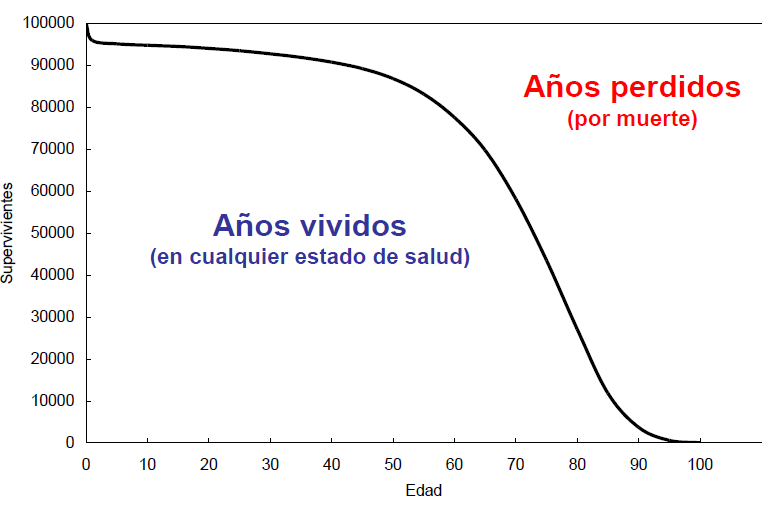
\includegraphics[width=0.6\linewidth]{grafi/teorico}
		\label{fig:teorico}
	\caption{APVP con l�mite constante.	Fuente: Manual 
		de Epidat.}
\end{figure}
\end{frame}
\begin{frame}
\frametitle{Ejemplo 6 (BOOTSTRAP) - APVP con $e_x$ como l�mite}
Es por esto que se propone utilizar el tercer supuesto 
planteado por \cite{Arriaga1996} obteniendo la 
siguiente ecuaci�n:
\pause
\begin{equation}
APVP = \sum_{x=0}^{\omega-1} e_{x} d_{x}.
\label{e:apvpmod}
\end{equation}
\pause
\begin{figure}[htbp]
\centering
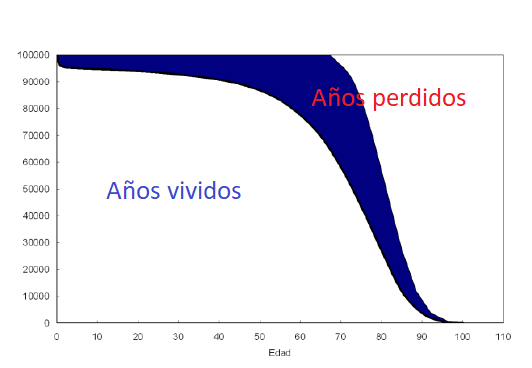
\includegraphics[width=0.5\linewidth]{grafi/teorico2}
\caption{APVP con $e_x$ como l�mite:	Fuente: Manual 
	de Epidat.}
\label{fig:teorico2}
\end{figure}
\end{frame}


\begin{frame}
\frametitle{Ejemplo 6 (BOOTSTRAP) Estimaci�n bootstrap del sesgo de un estimador}

\begin{block}{}
	A los efectos de introducir el m\'etodo bootstrap no param\'etrico, \cite{Scavino2020} y algunas de sus aplicaciones, se propone, en primer lugar, estimar el llamado \emph{sesgo} (bias) de un estimador ${\widehat{\theta}}_n = {\widehat{\theta}}_n(X_1, \ldots, X_n)$ de un par\'ametro $\theta=\theta(F)$, definido por
	
	\begin{equation}
	\label{sesgo}
	\text{Sesgo}(\widehat{\theta}_n) = E_F(\widehat{\theta}_n) 
	- \theta(F). 
	\end{equation}
\end{block}
\pause
\begin{block}{}
	El m\'etodo bootstrap no param\'etrico consiste esencialmente en la aplicaci\'on de dos pasos relacionados entre s\'{\i}, descritos a continuaci\'on para el caso de un estimador $\widehat{\theta}_n$ de $\theta$ que cumple el principio plug-in. \\ Dada la realizaci\'on $\mathbf{x} = (x_1, \ldots , x_n)$ de la MAS. $\mathbf{X} = (X_1, \ldots , X_n)$,
	
	\begin{itemize}
		\item \textbf{(paso 1)} sustituir la $F$ desconocida por la 
		distribuci\'on emp\'{\i}rica 
		${\mathbb{F}}_{n,\mathbf{x}}(x)$.
		\pause
		\item\textbf{(paso 2)} sustituir las variables aleatorias 
		i.i.d. de la distribuci\'on $F$ que aparecen en el 
		problema de inter\'es por muestras $\mathbf{X}^* = 
		(X_1^*, \ldots , X_n^*)$ generadas con reemplazo a 
		partir de la muestra original $\mathbf{X} = (X_1, 
		\ldots , X_n)$ por medio de la distribuci\'on 
		emp\'{\i}rica ${\mathbb{F}}_{n,\mathbf{x}}(x)$.
	\end{itemize}
	
\end{block}

\end{frame}

\begin{frame}
\frametitle{Ejemplo 6 (BOOTSTRAP) Procedimiento}
\begin{block}{}
	
	Para el c\'alculo aproximado de la estimaci\'on bootstrap 
	para sesgo  (\ref{sesgo}) de un estimador 
	$\widehat{\theta}_n$ de $\theta$ que cumple el principio 
	plug-in es necesario implementar un algoritmo  que plantean varios autores y que podr�a tener la siguiente estructura \cite{bootstrap2019}: 
	\pause
	
	\begin{enumerate}
		\item[1.] Registrar la realizaci\'on $\bf{x}$ de la 
		MAS $\bf{X}$.
		\item[2.] calcular la estimaci\'on de $\theta$ basada 
		en $\bf{x}$: ${\widehat{\theta}}_n(x_1, \ldots, x_n)$.
		\item[3.] generar $n$ observaciones de la 
		distribuci\'on emp\'{\i}rica 
		$\mathbb{F}_{n,\mathbf{x}}$, esto es, una 
		realizaci\'on $x_1^*, \ldots, x_n^*$.
		\item[4.] calcular la estimaci\'on 
		${\widehat{\theta}}_n(x_1^*, \ldots, x_n^*) = 
		\widehat{\theta}_n^*$.
		\item[5.] repetir $B$ veces los pasos 3 y 4, obteniendo 
		las estimaciones $\widehat{\theta}_{n,1}^*, \ldots, 
		\widehat{\theta}_{n,B}^*$.
		\item[6.] calcular la cantidad 
		\begin{equation} \label{estsesgoboot}
		\widehat{\text{Sesgo}}^*(\widehat{\theta}_n) = 
		\frac{1}{B} \sum_{j=1}^B  \widehat{\theta}_{n,j}^* - 
		{\widehat{\theta}}_n(x_1, \ldots, x_n) \,.
		\end{equation} 
	\end{enumerate}
	
\end{block}
\end{frame}
\begin{frame}
\frametitle{Distribuci\'on de los APVP para sexo Masculino}  

\begin{figure}
	\centering
	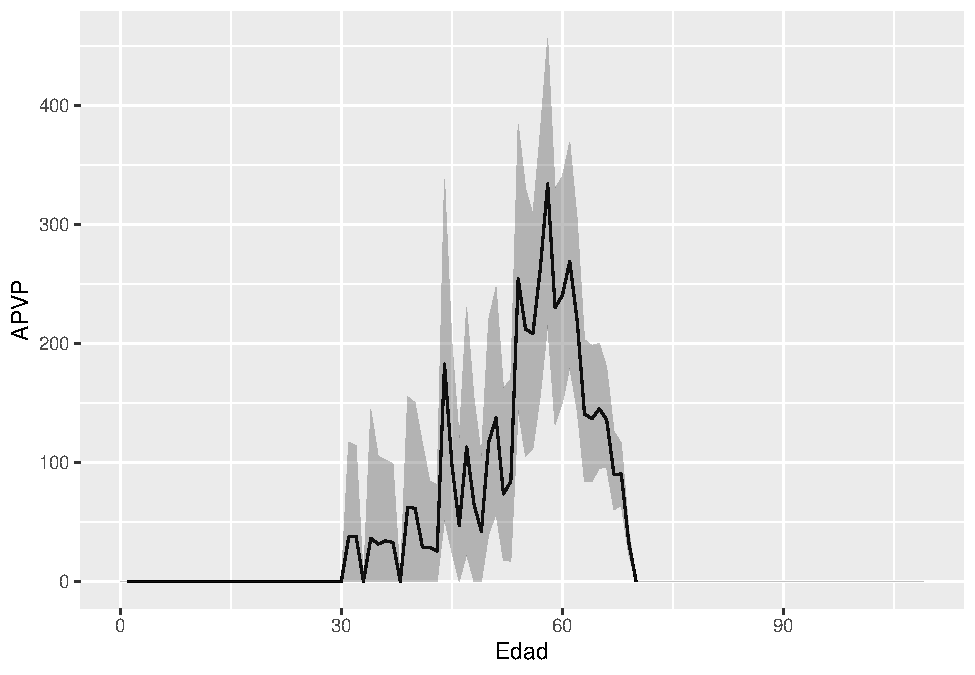
\includegraphics[width=0.8\linewidth]{grafi/unnamed-chunk-12-1.pdf}
	\caption{Distribuci\'on de los APVP para cada edad y 
		con una banda al $95\%$ de los
		cuantiles emp\'iricos, para el sexo Masculino y 
		edad 
		l\'imite $L=70$.}
	\label{fig:APVP2}	
\end{figure}
\end{frame}


\begin{frame}
\frametitle{En Resumen (1)}  
	\begin{itemize}
		\item En resumen a lo largo de estas situaciones vimos que deberemos saber usar t\'{e}cnicas de aproximaci\'{o}n para la resoluci\'{o}n de problemas mediante el uso de computadoras ya que en alg\'{u}n caso la soluci\'{o}n
		anal\'{i}tica es muy dif\'{i}cil cuando no imposible.
		\item 	Pero lo m\'{a}s importante es que las t\'{e}cnicas que usemos se ver\'{a}n mo\-dificadas ya que la matem\'{a}tica de la computadora es ''otra'' (recordar el ejemplo de
		la suma), con lo que deberemos aprender exactamente cual es el error que se comete y pensar en formas de c\'{a}lculos (algoritmos) f\'{a}ciles con resultados r\'{a}pidos (ejemplo de la evaluaci\'{o}n de polinomios).
	\end{itemize}
\end{frame}

\begin{frame}
\frametitle{En Resumen (2)}  
\begin{itemize}
	\item Por lo tanto vamos a necesitar de un lenguaje de  programaci\'{o}n y nosotros usaremos el \citep{Rcoreteam2022} aunque lo m\'{a}s importante no es cual sino que sepamos plantear nuestro problemas en t\'{e}rminos l\'{o}gicos de manera que la computadora sea capaz de realizar todas las mismas tares que nosotros
	har\'{i}amos en forma manual con la ayuda de una calculadora de bolsillo.
	\item   Componentes
	\begin{enumerate}
		\item \emph{T\'{e}cnicas de programaci\'{o}n}
		\item \emph{T\'{e}cnicas Num\'{e}ricas}
		\item \emph{Los m\'{e}todos de \textbf{SIMULACI\'ON}}
	\end{enumerate}\
\end{itemize}
\end{frame}

\begin{frame}
	\frametitle{Curso(1)} 
	\begin{figure}[htbp]
		\centering
		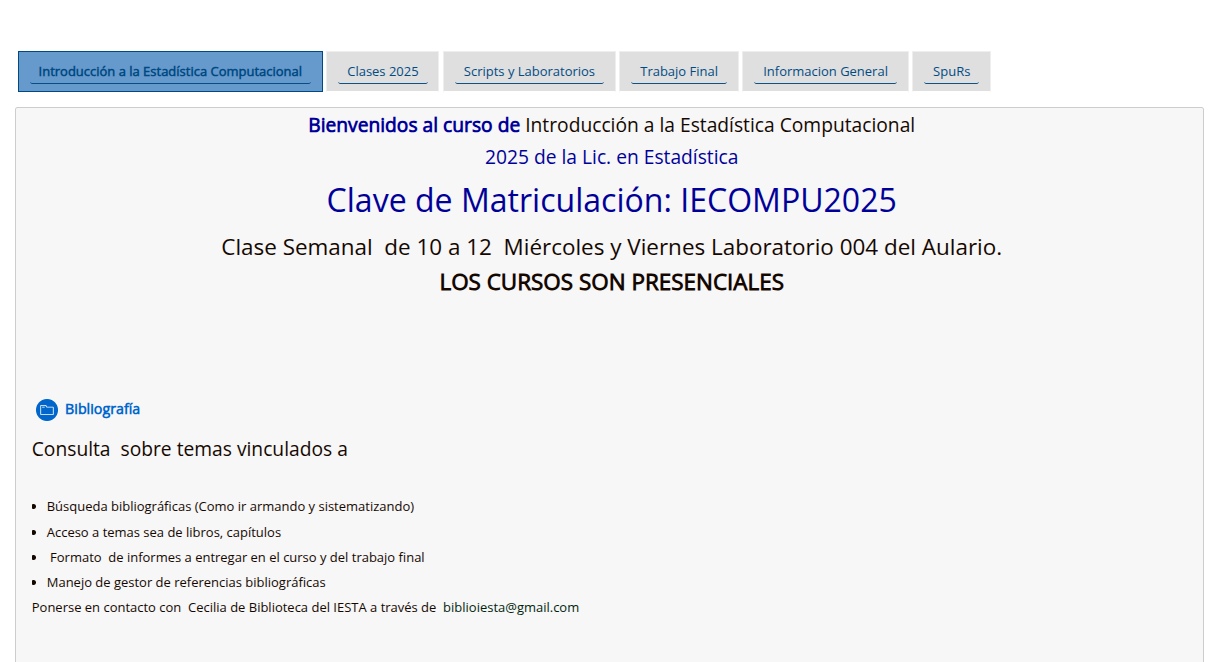
\includegraphics[width=0.90\textwidth]{grafi/curso1.png}
		\label{fig:curso1}
		\caption{Curso Introducci�n a la Estad�stica Computacional. Pesta\~na General}
	\end{figure} 
\end{frame}


\begin{frame}
	\frametitle{Curso(2)} 
	\begin{figure}[htbp]
		\centering
		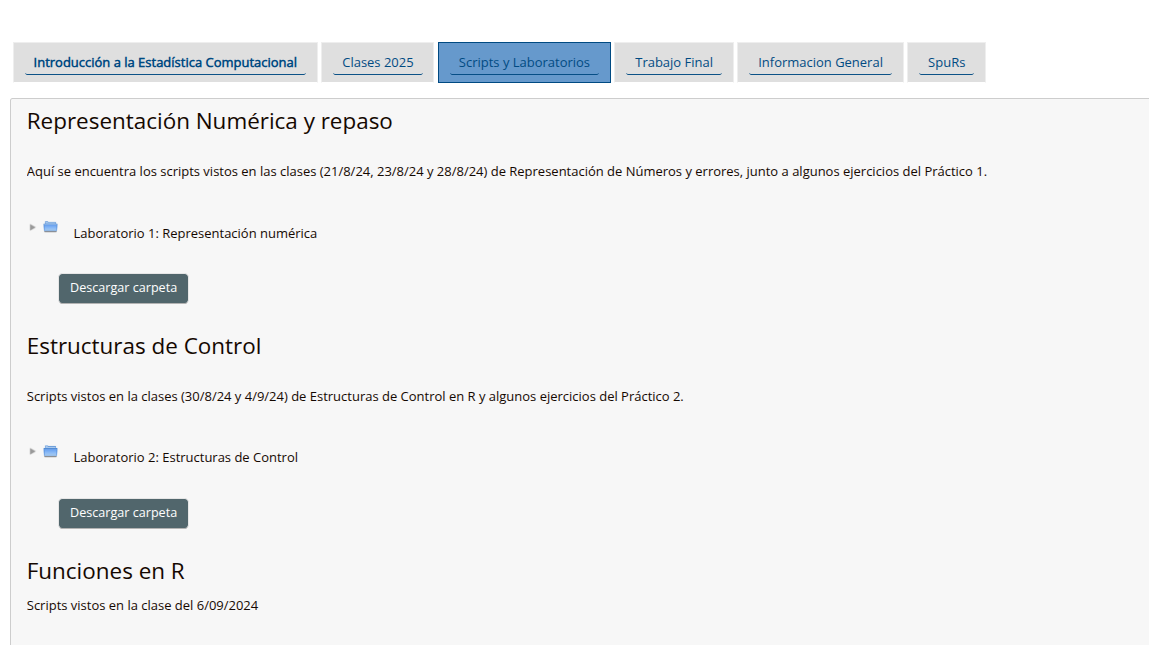
\includegraphics[width=0.90\textwidth]{grafi/curso2.png}
		\label{fig:curso2}
		\caption{Curso Introducci�n a la Estad�stica Computacional. Scripts}
	\end{figure} 
\end{frame}


\begin{frame}
	\frametitle{Curso(1)} 
	\begin{figure}[htbp]
		\centering
		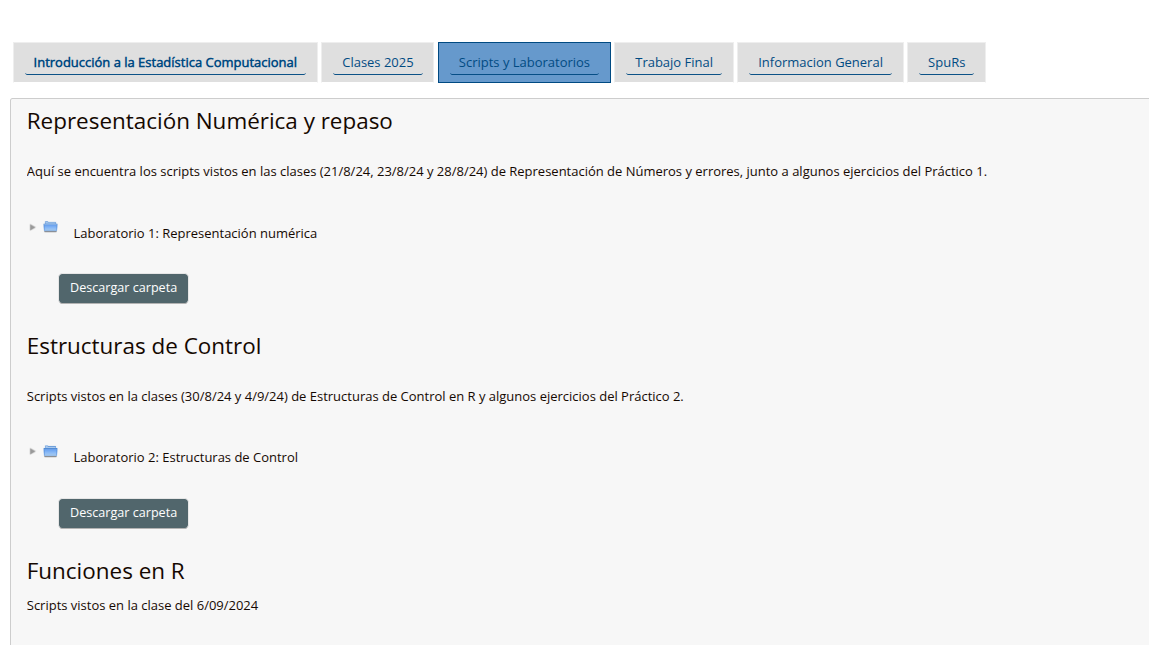
\includegraphics[width=0.90\textwidth]{grafi/curso2.png}
		\label{fig:curso3}
		\caption{Curso Introducci�n a la Estad�stica Computacional.Trabajo Final}
	\end{figure} 
\end{frame}

\begin{frame}
	\begin{center}
		\Huge{�Preguntas?}
	\end{center}
\end{frame}



\begin{frame}
	\begin{center}
		\Huge{Muchas Gracias}
	\end{center}
\end{frame}


\begin{frame}
\frametitle{Bibliograf\'ia}  
	\bibliographystyle{apalike}
	{\small 
	\bibliography{biblio/Taller_Montecarlo}}

\end{frame}



\end{document}
